% !TEX TS-program = Xe\LaTeX\ 
	% the above line of code forces THIS SCRIPT to compile with Xe\LaTeX\ , instead of \LaTeX\ .  This just provides more options.  
\documentclass[11pt]{article}
%Begin preamble (ie. info latex needs before you start your document).  
%%%%%%%%%%%%%%%%%%%%%%%%%%%%%%%%%%%%%%%%%%%%%%%%
\usepackage{geometry}                			% See geometry.pdf to learn the layout options. There are lots.
\geometry{a4paper}                   				% ... or a4paper or a5paper or ... 
%\geometry{landscape}               			% Activate for for rotated page geometry
%\usepackage[parfill]{parskip}    			% Activate to begin paragraphs with an empty line rather than an indent
\geometry{top=1.0in, bottom=1.0in, left=1.0in, right=1.0in}	%set margins (currently 1 inch on all sides.  Turn off to accept defaults (better for documents that will be turned into books).  
\usepackage{fullpage}					%Package forces latex to use more of the A4 page 
\usepackage{graphicx}					%Package required to include graphics		
\usepackage{amssymb}					%Package required to use some symbols 
\usepackage{epstopdf}					%Package required to convert this code into a pdf
\usepackage[tight,TABTOPCAP]{subfigure}	%Package used to ensure subfigures are oriented correctly
\usepackage{multirow}					%Package used for using 'merged rows' in tables
\usepackage{booktabs}					%Package used to make better formatted table, follows correct table format conventions.
\usepackage{threeparttable}				%Package to allow footnotes in tables.  
\usepackage{color}    					%Package used for adding colored text
\usepackage{lineno}       					%Package used for adding line numbers
\usepackage{placeins}
%\usepackage{"The font you want for the entire document"}  Options must be included in your distribution.  Try:  avant, bookman, chancery, charter, courier, helvet (helvetica), lucida, newcent (new century), palatino, pslatex, punk, times (time new roman), utopia
\usepackage[colorlinks]{hyperref}  					%Package that turns all lists of contents, lists of figures and lists of tables, and all intext references into hyperlinks sothe reader can click on them and it takes them to relevent part of the document.  (And all you had to do was type ONE LINE OF CODE!!!) Find the 'hyperref manual' online for how to adjust settings/options (eg [colorlinks] changes the color of all hyperlinks to various colored text).  
\usepackage{url}						%Package that allows the use of url's with 'special characters' that normally dont work.  
\DeclareGraphicsRule{.tif}{png}{.png}{`convert #1 `dirname #1`/`basename #1 .tif`.png}
%\pagestyle{empty}

\title{Latex Training Document} 			
\author{Tomas Remenyi}
\date{\today}                     			                  % Activate to display a given date or no date
%%%%%%%%%%%%%%%%%%%%%%%%%%%%%%%%%%%%%%%%%%%%%%%%
%End preamble
\begin{document}
\linenumbers  							%Must have \usepackage{lineno} added to preamble
\maketitle

\tableofcontents
\listoffigures
\listoftables

\newpage
I have now forced a new page.  Look at  the code.  

\section{First things first: What is it and how do I install \LaTeX\ !!!}  
\subsection{What is it?}
I don�t want reinvent the wheel... here is the link to the wiki book.
\\ \url{http://en.wikibooks.org/wiki/LaTeX/Introduction}

\subsection{How to install \LaTeX\ !!!}
I have re-invented the wheel for this one... sometimes you get a better wheel!

First of all, there are lots of different types of \LaTeX\  distributions.  To simplify your search process I will suggest you choose from the below(last updated , September, 3rd, 2011).  
\\ (I suggest following the instructions at this website if your having trouble with the install:
\\ \url{http://www.haptonstahl.org/latex/start_downloading.php})

\subsubsection{WINDOWS and LINUX users:} Download the latest version of Tex Live or MikTex (currently 2.8).  It should come with TeXWorks as the user interface.  \\ \url{http://docs.miktex.org/2.8/relnotes/}

\subsubsection{MAC users:}  Download the latest version of MacTeX.  This comes with TeXShop as the user interface (TeXWorks is unashamedly based on TeXShop.  TeXShop is older, and more developed, so at the moment is better. However, keep checking the net for comparisons.  If you plan to use multiple platforms (Mac, Linux and Windows, then use TeXWorks, so you only have to learn how to use one style).  \\ \url{http://www.tug.org/mactex/2009/}


\section{The absolute basics}
\subsection{How to create a document with ``hello world'' as the content~~} Go to this link \url{http://www.youtube.com/watch?v=kQl2XdBiWNE&feature=related} \\  I suggest saving the first document you create into a folder on the desktop called ``MyFirstTexDocument''.  This is designed for TexShop but most of this is applicable to TexWorks too.  


\section{TexWorks ethos video link}\url{http://www.youtube.com/watch?v=9-Z43CSPgM0}

\section{This is a section heading~~}  This is where the text goes in a section.  I will repeat this to create more words.  A few more words.  This is what happens when there is a really long sentence, or paragraph and how it looks on the page so you can see how it works.  I will repeat this to create more words. I will repeat this to create more words.  A few more words.  This is what happens when there is a really long sentence, or paragraph and how it looks on the page so you can see how it works.  I will repeat this to create more words. 


\subsection{This is a subsection heading~~}  This is where the text goes in a section.  I will repeat this to create more words.  A few more words.  This is what happens when there is a really long sentence, or paragraph and how it looks on the page so you can see how it works.  I will repeat this to create more words. I will repeat this to create more words.  A few more words.  This is what happens when there is a really long sentence, or paragraph and how it looks on the page so you can see how it works.  I will repeat this to create more words. 

\subsubsection{This is a subsubsection heading~~} This is where the text goes in a section.  I will repeat this to create more words.  A few more words.  This is what happens when there is a really long sentence, or paragraph and how it looks on the page so you can see how it works.  I will repeat this to create more words. I will repeat this to create more words.  A few more words.  This is what happens when there is a really long sentence, or paragraph and how it looks on the page so you can see how it works.  I will repeat this to create more words. 



\paragraph{This is a paragraph heading} with a few illustrative following paragraphs.   This paragraph is to show you how to insert new parargraphs with funky headings.  

And then how to make a normal paragraph too, with a different indent etc.  And then how to make a normal paragraph too, with a different indent etc.  And then how to make a normal paragraph too, with a different indent etc.  And then how to make a normal paragraph too, with a different indent etc.  And then how to make a normal paragraph too, with a different indent etc.   


\bigskip
I have created the space, or empty line, by using a command, see the code.    And then how to make a normal paragraph too, with a different indent etc.  And then how to make a normal paragraph too, with a different indent etc.  And then how to make a normal paragraph too, with a different indent etc.  And then how to make a normal paragraph too, with a different indent etc.  And then how to make a normal paragraph too, with a different indent etc.  And then how to make a normal paragraph too, with a different indent etc.  And then how to make a normal paragraph too, with a different indent etc.  And then how to make a normal paragraph too, with a different indent etc.  And then how to make a normal paragraph too, with a different indent etc.  And then how to make a normal paragraph too, with a different indent etc.  

And then how to make a normal paragraph too, with a different indent etc.  And then how to make a normal paragraph too, with a different indent etc.  And then how to make a normal paragraph too, with a different indent etc.  And then how to make a normal paragraph too, with a different indent etc.  And then how to make a normal paragraph too, with a different indent etc.  

\newpage
\section{How to make Figures and Tables}  
\LaTeX\ has a sensible, but very annoying, function that automatically locates your figures in the document where it believes is the best spot, NOT where you placed it in the text / code.    Sometimes getting the figure to be exactly where you want it in a long document is tricky.  However, because it does this, figures and tables are always located in the same relative positions throughout the entire document (e.g. top of the page) which gives the document a real sense of balance and continuity... It is still really annoying sometimes though...

To force \LaTeX\ to ignore this functionality sometimes, use either:\\
 \verb+ \begin{figure}[h] + where h=here\\
 or\\
 \verb+ \FloatBarrier + which forces all previous "floats" (figure or table environments) to be placed in the document before any of the following text / code.  


\begin{figure}[t] % I used `t' for top, instead of b=bottom, h=here or p=page of figures.  
\begin{center}
\includegraphics[width=0.8\textwidth]{50pinIsosurface0dbarAbsoluteSalintyWithFronts.png} %(NB:  if you have not got the figure in the same folder as your \LaTeX\  document, you will need to use the entire path name.)
\caption{This is how you make a figure}
\label{justafigure}
\end{center}
\end{figure}


\begin{figure}[t]
\begin{center}
\subfigure[This is a plot of \emph{Absolute Salinity} across a section of the ocean, x-axis is latitude,  y-axis is depth]{\includegraphics[height=0.25\textheight,width=0.48\textwidth]{EastSection_NtoS_250m_AbSal_100dpi.png}\label{sectionAbSal}}
\subfigure[This is a plot of \emph{Absolute Salinity} across the surface of the ocean around Tasmania in summer 2007, x-axis is longitude,  y-axis is latitude]{\includegraphics[height=0.25\textheight,width=0.48\textwidth]{50pinIsosurface0dbarAbsoluteSalintyWithFronts.png}\label{surfaceAbSal}}
\subfigure[This is a plot of \emph{dissolved aluminium} across the same section of the ocean as \ref{sectionAbSal}, x-axis is latitude,  y-axis is depth]{\includegraphics[height=0.25\textheight,width=0.48\textwidth]{EastSection_NtoS_250m_dAl_100dpi.png}\label{sectionDAl}}
\subfigure[This plot displays the effect of using a matrix elimination step during the analysis of a aluminium--lumogallion complex in a seawater sample]{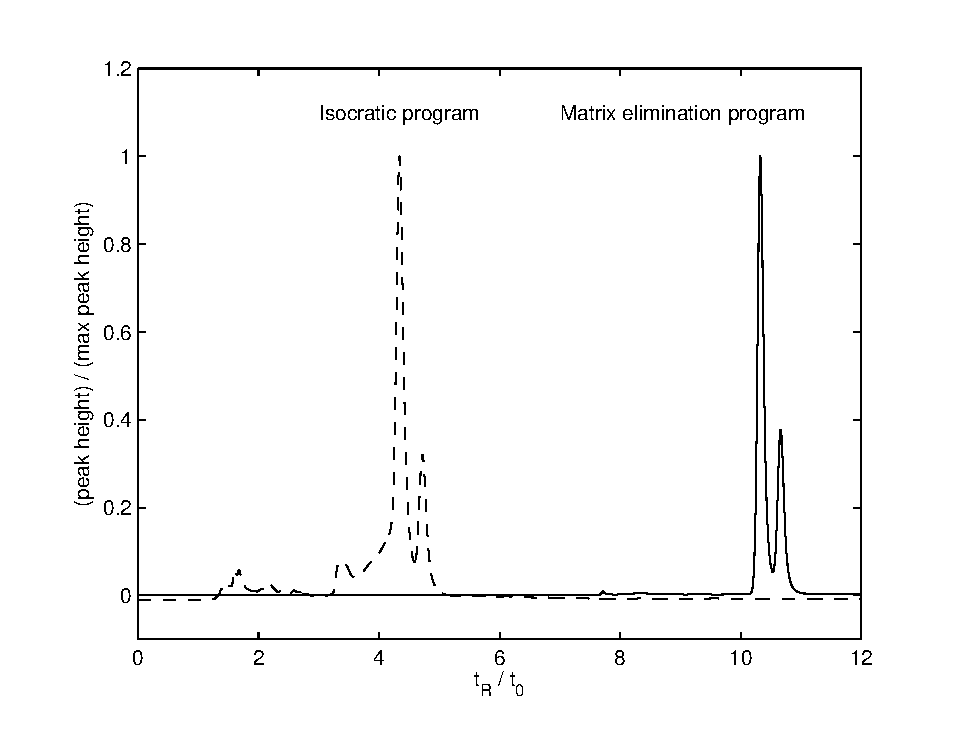
\includegraphics[height=0.25\textheight,width=0.48\textwidth]{isocratic_vs_gradient.eps}\label{isocVSgrad}}
\caption{This is how you do subfigures}
\label{subfigureexample}
\end{center}
\end{figure}

\begin{figure}[t]
\begin{center}
\includegraphics[height=0.25\textheight,width=0.48\textwidth]{EastSection_NtoS_250m_dAl_100dpi.png}
\includegraphics[height=0.25\textheight,width=0.48\textwidth]{EastSection_NtoS_250m_AbSal_100dpi.png}
\caption{This is how you get two pictures in the same figure on the same line}
\label{twopicturefigure}
\end{center}
\end{figure}

\begin{figure}[t]
\begin{center}
\includegraphics[height=0.25\textheight,width=0.48\textwidth]{EastSection_NtoS_250m_dAl_100dpi.png}\\
\includegraphics[height=0.25\textheight,width=0.48\textwidth]{EastSection_NtoS_250m_AbSal_100dpi.png}
\caption{This is how you get two pictures in the same figure one on top of the other}
\label{twopicturefigure}
\end{center}
\end{figure}

\FloatBarrier


\section{How to use \textbf{bold} and \textit{italics}, and \emph{emphasize}} 
\subsection{Bold~~}  This is where the text goes in a subsection. \begin{bf} I will repeat this to create more words.  \end{bf}   I will repeat this to create more words. I will repeat this to create more words.  
\subsection{Italize~~} A few more words.  This is what happens when there is a really long sentence, or paragraph and how it looks on the page so you can see how it works. \begin{it} A few more words.  This is what happens when there is a really long sentence, or paragraph and how it looks on the page so you can see how it works.  I will repeat this to create more words. \end{it}A few more words.  This is what happens when there is a really long sentence, or paragraph and how it looks on the page so you can see how it works.  I will repeat this to create more words. 
\subsection{Emphasize~~} A few more words.  \emph{This is what happens} when there is a really long sentence, or paragraph and how it looks on the page so you can see how it works. \begin{it} Check the \textbf{\emph{source code}} for the various ways these \emph{commands} can be \textbf{used}.  Check the source code for the \textbf{various} ways \emph{these} commands can be used.  \end{it}A few more words.  This is what happens when there is a really long sentence, or paragraph and how it looks on the page so you can see how it works.  I will repeat this to create more words. 
\section{How to add different coloured text~~}
 \begin{color}{red}NB:  Note the different code I have used to end the line here!!!! I have repeated it below as well.  It shows how to make a newline, without makeing a new paragraph\end{color} \\
 \begin{color}{blue} And the color change I have used.  \end{color}  
However this is how you make a normal parargraph.  However this is how you make a normal parargraph.  However this is how you make a normal parargraph.  However this is how you make a normal parargraph.  

However this is how you make a normal parargraph.  However this is how you make a normal parargraph.  However this is how you make a normal parargraph.  However this is how you make a normal parargraph.  However this is how you make a normal parargraph.  However this is how you make a normal parargraph.   

\begin{color}{red}NB:  Note where this sentence is in the code, and where it is relative to all the figures in the document.  \LaTeX\  decides where figures work best, given the space available in the document.  \end{color}


\newpage %Put a percentage sign (%) at the start of this line, typeset the document again (once you have \LaTeX\  up and running) and see what happens... 
I have now forced a new page.  Look at  the code.  

\bigskip
Note where the table is in the code, and where it is in the document.  Tables and figures are called \emph{floats}, and so they are `floating' to the best position for the readers eye-flow while reading.  


\begin{table}[t]
\begin{threeparttable}[b] 
\caption{This is how you make a table.  }
\begin{center}
\begin{tabular}{c c c c}	%these are vertical lines (shift-backslash key) and the letter 'c' for centre alignment (alternatives are 'r' for right and 'l' for left).  
\toprule
&\multicolumn{3}{r}{\textbf{Multiple columns are done like this}} \\
\midrule
\multirow{5}{*}{\textbf{Multiple rows, like this}}& aardvark & bison & cat \\
&dog &emu &fish\\
&giraffe& horse &iguana\\
& jaguar &kite& lizard \\
&&&\\
\textbf{Footnotes in tables}\tnote{1} & Are done & using the & \emph{threeparttable} package\tnote{2}, \tnote{3}\\
\bottomrule
\end{tabular}
\begin{tablenotes}
\item[1]  Footnotes in tables should be avoided.  Conventions for good table formatting is summarised in the \emph{booktabs} package, and I recommend you use that to produce your tables.
\item[2]  However sometimes they are necessary, and you need to use the\\ \emph{threeparttable} package for that.  
\item[3]  For tables with a lot of content, or that already exist in excel, I suggest investgating how to use the ``OpenOffice'' plugin called ``Calc2Latex''. This simplifies the construction and alteration of content in the latex code you need in a table.  
\end{tablenotes}
\end{center}
\label{howtomakeatable}
\end{threeparttable}
\end{table}%

%The main things to note are, to span multiple columns in a latex table you just use \multicolumn followed by the number of columns to span and how you want it positioned, e.g. l for left, r for right, c for centered. 
% Spanning multiple rows in a latex table is the same, except YOU NEED TO USE:  "\usepackage{multirow}" in the preamble (at the top), and using \multirow followed by the number of rows to span, and how you would like it positioned. * basically means best fit. Remember that the first element/column of each row needs to be empty, since you have some piece of information spanning multiple rows.





\section{Making lists (bullets points and the like...)}Below is a few examples of making lists... There are many more styles.    

\begin{itemize}
\item  Point 1
\item Point 2
\item Point 3
\begin{enumerate}
\item Point 3.1
\item another point 3.2
\item another 3.x
\begin{itemize}
\item Some extra 3.x.a
\item Some extra 3.x.1
\item Some extra 3.x.zebra
\end{itemize}
\item some more points
\item some more points
\end{enumerate}
\item some more points
\item some more points\item some more points
\end{itemize}



\section{How you do equations}
\subsection{Puting equations in the text~~}  This is how you do equations in a sentence using the Math environment:  $a=b+7c^2 - d_{testing} \times 15e^{2^{h}_i} \rightarrow 2f_{2\Delta}$.  

However, this equation is cut in half by the end of the line on the page.  So to force and `end of line', I will put in a `newline' command = \begin{verbatim} \\ \end{verbatim}  So that again is:  \\
This is how you do equations in a sentence using the Math environment: \\ $a=b+7c^2 - d_{testing} \times 15e^{2^{h}_i} \rightarrow 2f_{2\Delta}$ \\
\subsection{Numbering equations~~}  

This is how you give equations a number and a lot of space!!
\begin{equation}
\rho + \delta - \frac{345^{x^2 } + \theta \times \Omega_{x-1}}{rarely\ you\ may\ want\ (some\ written\ text\ \times \pi + \chi)}
\label{howtomakeanumberedequation}
\end{equation}


\subsection{Refer to your figures and tables in the text}  I will now reference the figures again.  I added a command inside each table or figure environment that was \begin{verbatim} \label{RandomNameForFigure} \end{verbatim}.  I now use \begin{verbatim} \ref{RandomNameForFigure}\end{verbatim} to refer to each figure, subfigure or table in the text.  

When used it look s like this:  So I refer to what is in table \ref{howtomakeatable}, and the figures \ref{justafigure} and \ref{twopicturefigure}, there are no subfigures.  However in figure \ref{subfigureexample} there are subfigures, such as \ref{sectionDAl}, and the rest...

\section{Which spell checker to use....}
Go online and find the most appropriate for your platform.  

\subsection{Suggested spell checker for Mac OSX}  I use a Mac, with OSX so I use CocoaSpell (its awesome).  It has a dictionary the includes all of the latex commands (like \begin{color}{blue}\textbackslash section\end{color}), which is really handy.  

\subsection{Suggested spell checker for Windows}  Unknown...

\subsection{Suggested spell checker for Linux}  If your using linux, you can probably figure out how to find the one that suits you best, based on the distribution and form of \LaTeX\  your using...

\section{How to cite references in \LaTeX\ }

This is how you cite references in latex.  It is very like using endnote, so if you know how to do that, find the referencing software for your platform (I suggest JabRef, operates on all platforms, very versatile, lots of functionality), install it, and use it!   \\

However, if you have never used any referencing software (THEN START!!!), you will need a little bit of learning to get it to work.  Its easy and straight forward, but outside of the scope of this tute.  If you need help ask me.  
\subsection{This is just a small example of how you reference sources.}
First person to suggest humans may effect climate was Fourier \cite{fourier1824}.  The first person to suggest CO$_2$ may trap a large amount of heat per molecule was Tyndall \cite{tyndall1861} (John Tyndall is a legend, if you havent heard of him, look it up on the net).  
Andy Bowie is my supervisor and he has written scientific papers \cite{bowie2002} \cite{bowie2007}.  
Thomas Trull is my old boss and he has also written some papers \cite{trull2008} \cite{trull2008a}.  
Juliette Tria did some work on her PhD, and her papers effectively explain what I was trying to do in mine \cite{tria2008a} \cite{tria2008b}.  
Stefane Blain was nice enough to put me on his paper after I participated in an oceanographic voyage from Reunion Island to Kerguelen Island \cite{blain2007}.  

\section{Journal article templates}
Elesvier Journals (most of them)\\
\url{http://www.elsevier.com/framework_authors/misc/journal_refstyles.pdf}
(please send myself or Spoon the links to any other repositories you find)

\section{More info}
NB:  Copy and paste websites from the .pdf, \textbf{NOT} from the code.  You can just click on them too.  (Disclaimer:  some of these might be too old, I have not recently checked them). 
\subsection{Cheat sheet of common commands}  This will be useful once you get used to using \LaTeX\ .  \\
\url{http://www.stdout.org/~winston/latex/latexsheet.pdf}
\subsection{User Manual}
There are heaps online, start the home website and go from there: \\
\url{http://www.latex-project.org} \\ A good online guide written in `real person' instead of programmer-speak is :  \\ 
 \url{http://www.haptonstahl.org/latex/index.php}
\subsection{Find Latex symbols here}  Symbols used in latex can be found at these sites:  \\
\url{http://omega.albany.edu:8008/Symbols.html}\\
\url{http://www.artofproblemsolving.com/Wiki/index.php/LaTeX:Symbols}\\
\url{http://www.ctan.org/tex-archive/info/symbols/comprehensive/symbols-a4.pdf}\\
\subsection{How to import excel spreadsheets \\(but I would sugest using OpenOffice with the Calc2Latex plugin)}
See this website:  \\
\url{http://www.mackichan.com/index.html?techtalk/v30/30ts71.htm~mainFrame} 
\subsection{How to use `R' (an open-source statistics package) with/in latex.}
See this website:  \\
\url{http://www.stat.umn.edu/~charlie/Sweave/}\\This would be useful if you are doing regular reports using the same stats each time period.  
\subsection{Anything else, consult the Oracle of Google...}
Use real english into google after the keyword ``latex'':  \\
i.e. Type into the google search window   ``latex how do I make a figure" or ``latex figure'' or ``latex \emph{whatever you want to know}''.  Just try heaps of different synonyms for the thing you want.  


\bibliographystyle{unsrt} %Set the style you want your references to use.  
\bibliography{latex_training_document_bibliography} %set the library of references you want to use.  (NB:  if you have not got the library in the same folder as your \LaTeX\  document, you will need to use the entire path name.)

\end{document}  